\chapter{Chain Of Responsibility模式}
\section{责任链模式的概念}
\subsection{定义}
责任链(Chain of Responsibility)模式的定义:为了避免请求发送者与多个请求处理者耦合在一起,将所有请求的处理者通过前一对象记住其下一个对象的引用而连成一条链;当有请求发生时,可将请求沿着这条链传递,直到有对象处理它为止。
\\ 注:在责任链模式中,客户只需要将请求发送到责任链上即可,无须关心请求的处理细节和请求的传递过程,所以责任链将请求的发送者和请求的处理者解耦了。
\subsection{优点}
\begin{enumerate}
	\item 降低了对象之间的耦合度。该模式使得一个对象无须知道到底是哪一个对象处理其请求以及链的结构,发送者和接收者也无须拥有对方的明确信息;
	\item 增强了系统的可扩展性。可以根据需要增加新的请求处理类,满足开闭原则;
	\item 增强了给对象指派职责的灵活性。当工作流程发生变化,可以动态地改变链内的成员或者调动它们的次序,也可动态地新增或者删除责任;
	\item 责任链简化了对象之间的连接。每个对象只需保持一个指向其后继者的引用,不需保持其他所有处理者的引用,这避免了使用众多的 if 或者 if···else 语句;
	\item 责任分担。每个类只需要处理自己该处理的工作,不该处理的传递给下一个对象完成,明确各类的责任范围,符合类的单一职责原则。
\end{enumerate}
\subsection{缺点}
\begin{enumerate}
	\item 不能保证每个请求一定被处理。由于一个请求没有明确的接收者,所以不能保证它一定会被处理,该请求可能一直传到链的末端都得不到处理;
	\item 对比较长的职责链,请求的处理可能涉及多个处理对象,系统性能将受到一定影响;
	\item 职责链建立的合理性要靠客户端来保证,增加了客户端的复杂性,可能会由于职责链的错误设置而导致系统出错,如可能会造成循环调用。
\end{enumerate}
\subsection{责任链模式的角色}
\begin{enumerate}
	\item Handler处理者:定义一个处理请求的接口,包含抽象处理方法和一个后继连接。
	\item ConcreteHandler具体处理者:实现抽象处理者的处理方法,判断能否处理本次请求,如果可以处理请求则处理,否则将该请求转给它的后继者。
	\item Client请求者:创建处理链,并向链头的具体处理者对象提交请求,它不关心处理细节和请求的传递过程。
\end{enumerate}
\subsection{应用场景}
\begin{enumerate}
	\item 有多个对象可以处理一个请求,哪个对象处理该请求由运行时刻自动确定。
	\item 可动态指定一组对象处理请求,或添加新的处理者。
	\item 在不明确指定请求处理者的情况下,向多个处理者中的一个提交请求。
\end{enumerate}
\section{责任链模式实现——例一}
\begin{table}
	\begin{tabular}{|l|l|}
		\hline
		名字&说明\\
		\hline
		Trouble&表示发生问题的类。\\
		\hline
		Support&用来解决问题的抽象类\\
		\hline
		NoSupport&用来解决问题的具体类(永远不处理)\\
		\hline
		LimitSupport&用来解决问题的具体类(解决编号小于指定编号)\\
		\hline
		OddSupport&用来解决问题的具体类(奇数编号)\\
		\hline
		SpecialSupport&用来解决问题的具体类(指定编号)\\
		\hline
		Main&形成责任链,测试类\\
	\end{tabular}
\end{table}
\begin{figure}[!h]
	\centering
	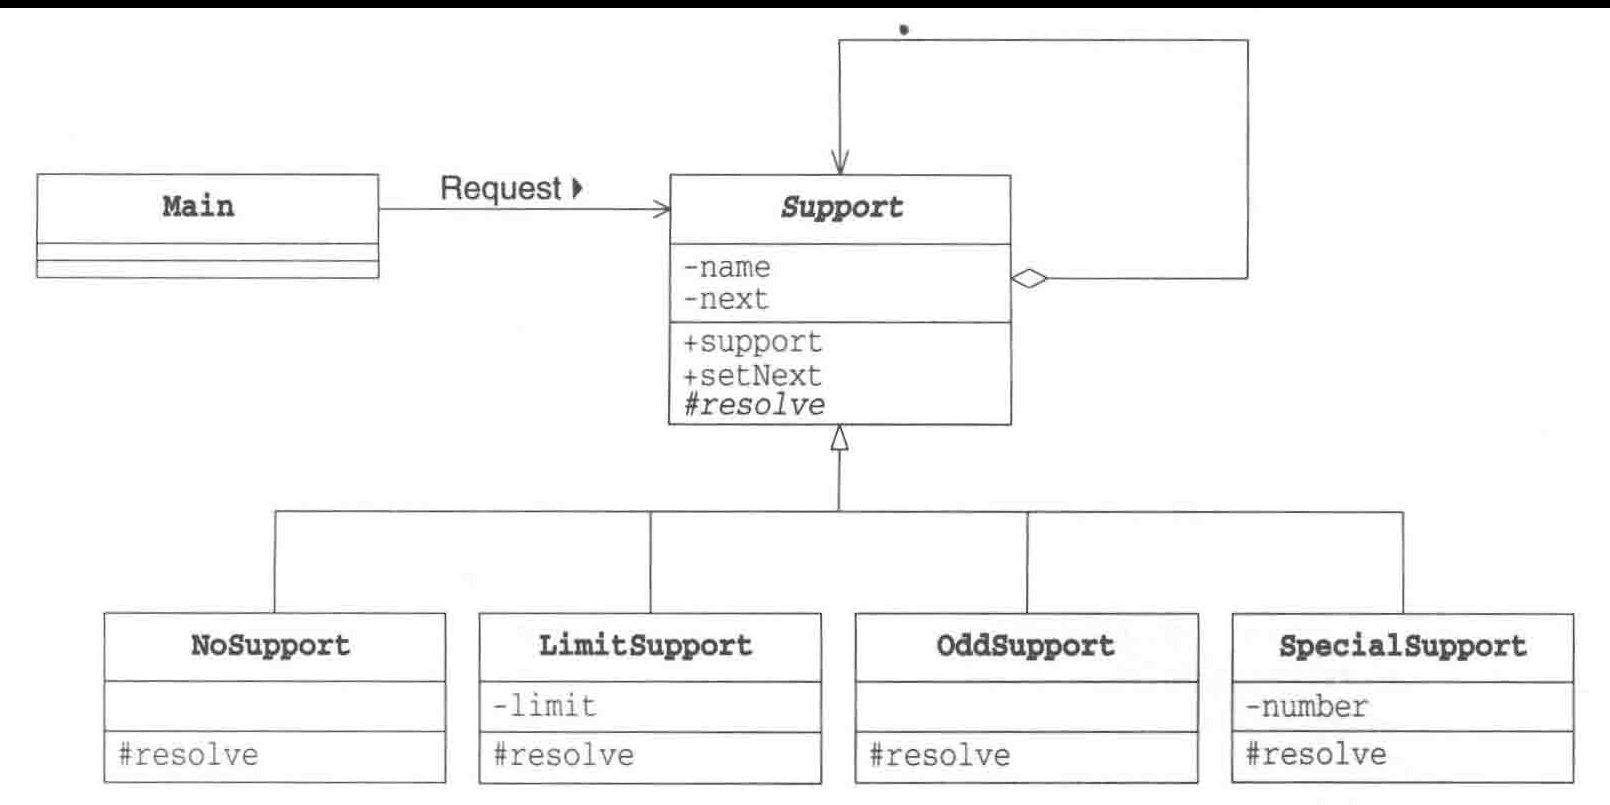
\includegraphics[width=\textwidth]{image/14-1}
	\caption{责任链模式的结构图}
\end{figure}
\begin{lstlisting}
//问题类,具有问题编号,编号是职责链处理的依据
public class Trouble {
	private int number;
	public Trouble(int number) {
		this.number = number;
	}
	public int getNumber() {
		return number;
	}
	public String toString() {
		return "[Trouble " + number + "]";
	}
}
\end{lstlisting}
\begin{lstlisting}
//解决问题德抽象类
public abstract class Support {
	//实例的名字
	private String name;
	//下一个处理人员
	private Support next;
	public Support(String name) {
		this.name = name;
	}
	public Support setNext(Support next) {
		this.next = next;
		return next;
	}
	public final void support(Trouble trouble) {
		if (resolve(trouble)) {
			done(trouble);
		} else if (next != null) {
			next.support(trouble);
		} else {
			fail(trouble);
		}
	}
	public String toString() {
		return "[" + name + "]";
	}
	//解决问题的办法
	protected abstract boolean resolve(Trouble trouble);
	//解决
	protected void done(Trouble trouble) {
		System.out.println(trouble + " is resolved by" + this + ".");
	}
	//未解决
	protected void fail(Trouble trouble) {
		System.out.println(trouble + " cannot be resolved.");
	}
}
\end{lstlisting}
\begin{lstlisting}
//永远不解决问题
public class NoSupport extends Support {
	public NoSupport(String name) {
		super(name);
	}
	protected boolean resolve(Trouble trouble) {
		return false;
	}
}
\end{lstlisting}
\begin{lstlisting}
//只解决编号小于 limit 的问题
public class LimitSupport extends Support {
	private int limit;
	public LimitSupport(String name, int limit) {
		super(name);
		this.limit = limit;
	}
	protected boolean resolve(Trouble trouble) {
		if (trouble.getNumber() < limit) {
			return true;
		} else {
			return false;
		}
	}
}
\end{lstlisting}
\begin{lstlisting}
//只解决奇数编号问题
public class OddSupport extends Support {
	public OddSupport(String name) {
		super(name);
	}
	protected boolean resolve(Trouble trouble) {
		if (trouble.getNumber() % 2 == 1) {
			return true;
		} else {
			return false;
		}
	}
}
\end{lstlisting}
\begin{lstlisting}
//只解决指定编号的问题
public class SpecialSupport extends Support {
	private int number;
	public SpecialSupport(String name, int number) {
		super(name);
		this.number = number;
	}
	protected boolean resolve(Trouble trouble) {
		if (trouble.getNumber() == number) {
			return true;
		} else {
			return false;
		}
	}
}
\end{lstlisting}
\begin{lstlisting}
public class Main {
	public static void main(String[] args) {
		Support alice = new NoSupport("ALice");
		Support bob = new LimitSupport("Bob", 100);
		Support charlie = new SpecialSupport("Charlie", 429);
		Support diana = new LimitSupport("Diana", 200);
		Support elmo = new OddSupport("Elem");
		Support fred = new LimitSupport("Fred", 300);
		
		alice.setNext(bob).setNext(charlie).setNext(diana).setNext(elmo).setNext(fred);
		for (int i = 0; i < 500; i += 33) {
			alice.support(new Trouble(i));
		}
	}
}
\end{lstlisting}
\section{责任链模式实现——例二}
\begin{figure}[!h]
	\centering
	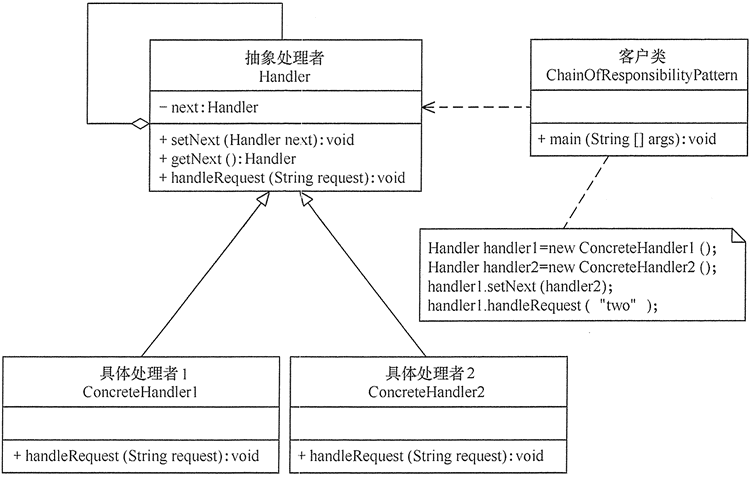
\includegraphics[width=0.8\textwidth]{image/14-2}
	\caption{责任链模式的结构图}
\end{figure}
\begin{figure}[!h]
	\centering
	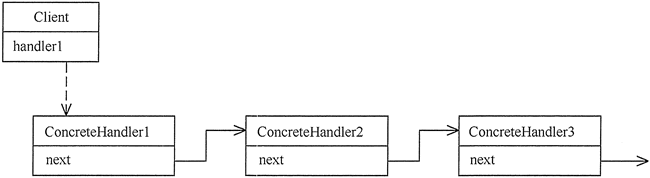
\includegraphics[width=0.8\textwidth]{image/14-3}
	\caption{责任链}
\end{figure}
\begin{lstlisting}
//抽象处理者角色
abstract class Handler {
	private Handler next;
	public void setNext(Handler next) {
		this.next = next;
	}
	public Handler getNext() {
		return next;
	}
	//处理请求的方法
	public abstract void handleRequest(String request);
}
\end{lstlisting}
\begin{lstlisting}
//具体处理者角色1
class ConcreteHandler1 extends Handler {
public void handleRequest(String request) {
if (request.equals("one")) {
System.out.println("具体处理者1负责处理该请求!");
} else {
if (getNext() != null) {
getNext().handleRequest(request);
} else {
System.out.println("没有人处理该请求!");
}
}
}
}

//具体处理者角色2
class ConcreteHandler2 extends Handler {
	public void handleRequest(String request) {
		if (request.equals("two")) {
				System.out.println("具体处理者2负责处理该请求!");
		} else {
			if (getNext() != null) {
				getNext().handleRequest(request);
			} else {
				System.out.println("没有人处理该请求!");
			}
		}
	}
}
\end{lstlisting}
\begin{lstlisting}
public class ChainOfResponsibilityPattern {
	public static void main(String[] args) {
		//组装责任链
		Handler handler1 = new ConcreteHandler1();
		Handler handler2 = new ConcreteHandler2();
		handler1.setNext(handler2);
		//提交请求
		handler1.handleRequest("two");
	}
}
\end{lstlisting}
\begin{lstlisting}
//output
具体处理者2负责处理该请求!
\end{lstlisting}
\section{模式扩展}
\begin{enumerate}
	\item 纯的职责链模式:一个请求必须被某一个处理者对象所接收,且一个具体处理者对某个请求的处理只能采用以下两种行为之一:自己处理(承担责任);把责任推给下家处理。
	\item 不纯的职责链模式:允许出现某一个具体处理者对象在承担了请求的一部分责任后又将剩余的责任传给下家的情况,且一个请求可以最终不被任何接收端对象所接收。
\end{enumerate}
\section{思路扩展}
\begin{enumerate}
	\item 弱化了请求的人和处理请求人之间的关系(优点),否则会降低可复用组件的独立性。
	\item 可以动态地改变职责链。
	\item 专注于自己的工作。
	\item 会导致延迟吗?虽然提高了灵活性,但会导致延迟。
\end{enumerate}
\section{相关设计模式}
\begin{enumerate}
	\item Composite模式:Handler经常使用Composite模式;
	\item Command向Handler发送请求。
\end{enumerate}